\documentclass[11pt]{article}
\usepackage[T1]{fontenc}
\usepackage{lmodern}
\usepackage[margin=1in]{geometry}
\usepackage{amsmath,amssymb,amsthm,mathtools}
\usepackage{graphicx,booktabs,array,microtype}
\usepackage[numbers,sort&compress]{natbib}
\usepackage[colorlinks=true,linkcolor=blue,citecolor=blue,urlcolor=blue]{hyperref}
\newtheorem{theorem}{Theorem}[section]
\newtheorem{lemma}[theorem]{Lemma}
\newtheorem{proposition}[theorem]{Proposition}
\newtheorem{corollary}[theorem]{Corollary}
\newcommand{\ReH}{\operatorname{Re}_{\!H}}
\newcommand{\ImH}{\operatorname{Im}_{\!H}}
\newcommand{\dd}{\,\mathrm{d}}
\newcommand{\ey}{\mathbf e_y}
\newcommand{\ex}{\mathbf e_x}
\newcommand{\ez}{\mathbf e_z}
\newcommand{\uvec}{\mathbf u_\theta}
\newcommand{\ip}[2]{\langle #1,#2\rangle}
\newcommand{\norm}[1]{\lVert #1\rVert}
\newcommand{\abs}[1]{\lvert #1\rvert}
\title{Unit Supremum of Absorption Asymmetry at Prescribed Extinction\\for Compact Reciprocal Dielectrics}
\author{Daniel Wang\\McMaster University\\\href{mailto:denialk391@gmail.com}{\texttt{denialk391@gmail.com}}
\and Junjie Zheng\\Columbia University\\\href{mailto:zjj2785@gmail.com}{\texttt{zjj2785@gmail.com}}}
\hypersetup{pdfauthor={Daniel Wang and Junjie Zheng},pdftitle={Unit Supremum of Absorption Asymmetry at Prescribed Extinction for Compact Reciprocal Dielectrics}}
\date{17 October 2026}
\begin{document}
\maketitle
\begin{abstract}
Reciprocity equates the extinction cross sections for opposite real linearly polarized plane waves, while permitting different absorption and scattering. At a fixed vacuum wavenumber $k>0$, we prove that the supremum of the absorption difference divided by common extinction is one at every exactly prescribed extinction $E_*>0$. The construction uses finite compact two-layer local anisotropic nonmagnetic dielectrics satisfying arbitrary fixed caps $P>1$ and $Q>0$, with $I\preceq\ReH\varepsilon\preceq PI$ and $0\prec\ImH\varepsilon\preceq QI$ in each layer. Every individual body has asymmetry strictly below one. The key step is an aperture limit uniform after factoring out the squared sine of the material rotation angle, including its zero-angle auxiliary limit. This permits the coupling angle to decrease as the aperture grows while extinction remains fixed. Positive isotropic loss is then added, and continuity permits exact retuning to the target. The approximating sequence has no common geometric resource bound or positive loss floor, and no bandwidth guarantee is asserted. The contribution is the controlled compact Maxwell realization at prescribed extinction. An accompanying Lean 4 formalization verifies the main existence and supremum statements and physical power identities; its verification and review scope are specified separately.
\end{abstract}

\section{Introduction and relation to OQ7}\label{sec:intro}
Open Question 7 in the tutorial of Miller and Monticone asks for fundamental limits on the redistribution between absorption and scattering under time-reversed illumination \citep{MillerMonticone2026}. A normalization, illumination class, and resource class are needed to turn that question into a theorem. Here the normalization is the common dimensional plane-wave extinction, the illumination pair is opposite real linear polarization in vacuum, and the objects are local reciprocal dielectric bodies at one frequency.

The result is an existence and supremum theorem. It states that a finite object can have exactly any prescribed positive extinction and an absorption difference arbitrarily close to that extinction, while its real permittivity and loss obey fixed pointwise upper bounds. It establishes neither a finite-resource optimum nor finite-bandwidth performance. The same material tensor is used in both experiments, and scattering includes the whole outgoing sphere and both polarizations.

At a fixed coupling angle, enlarging a planar-like aperture increases extinction proportionally to area. A fixed-stack aperture limit therefore does not suffice to prescribe total extinction. The exact rotation factorization and uniform normalized aperture theorem below permit the coupling angle to decrease while the aperture grows. Green-operator and localization arguments justify this passage for actual finite Maxwell bodies. Dipole optimization, scalar thickness laws, fixed-resource bounds, and quartic small-size results have different hypotheses and are outside the present proof.

\section{Prior work and the precise contribution}\label{sec:prior}
Reciprocal extinction equality and directional absorption are established facts. Sounas and Al\`u derived opposite-incidence extinction symmetry and its implications for scattering manipulation \citep{SounasAlu2014}. Hopkins and coauthors obtained directional absorption and scattering at equal extinction through modal interference in reciprocal particles \citep{Hopkins2015}. Power conservation gives the passive bound used here, and the optical theorem gives strict nonattainment for compact bodies.

Polarization conversion combined with selective attenuation also has established precedents. Armitage develops reciprocity constraints for Jones matrices and discusses a polarizer--waveplate example \citep{Armitage2014}. Khurgin and coauthors demonstrate reciprocal asymmetric polarization switching using selective attenuation and imperfect waveplates, including passive experiments \citep{Khurgin2021}. Thin bianisotropic absorbers and metasurfaces provide further examples of distinct opposite-side responses \citep{Radi2013,Yazdi2015}. M\'a\~nez-Espina and coauthors derive maximum directional absorptance difference in a reciprocal bianisotropic metasurface model and verify its predictions with full-wave simulations \citep{ManezEspina2026}. Kononchuk and coauthors combine selective attenuation with magnetic Faraday rotation in a layered-sheet isolator \citep{Kononchuk2019}; its complete device is magnetically nonreciprocal. These constructions must be compared with local nonmagnetic dielectric volumes under their respective constitutive and geometric assumptions.

Efficiency and response bounds clarify the resource requirements. Andersen and Frandsen show that receiving-antenna absorption divided by absorption plus total scattering can approach one at a directivity-dependent cost \citep{AndersenFrandsen2005}. Schab and collaborators formulate absorption--scattering tradeoffs with prescribed losses and material parameters \citep{Schab2020}, while Khurgin and Sun analyze loss scaling in resonant metal--dielectric structures \citep{KhurginSun2011}. Sounas and Al\`u derive multiport and free-space response bounds, including a stated extension to loss through additional channels \citep{SounasAlu2017}. These results constrain related responses but do not themselves construct the present opposite-incidence family at every prescribed extinction under arbitrary fixed dielectric caps.

For the finite-to-planar passage, Gao, Yang, and Kattawar study polarized extinction of plates with large aspect ratios \citep{Gao2013}. Gustafsson and coauthors derive planar extinction and scattered-transmission identities for periodic slabs \citep{Gustafsson2012}. Windowed Green-function methods treat layered backgrounds \citep{Bruno2016,Arrieta2022}, and volume-integral formulations supply the singular-kernel and radiation framework \citep{YurkinMishchenko2018,MishchenkoYurkin2018}. A computational window in an infinite-interface equation differs from literal truncation of a material body. Here smooth windows enter only trial currents; the final material aperture remains sharp.

Mann and Al\`u's conference abstract announces maximal directional absorption for bianisotropic dipolar particles \citep{MannAlu2023}. It is direct prior art for the qualitative extremal phenomenon, although its full equations, normalization and possible equivalence to a compact dielectric realization remain unverified. The contribution established here is the uniform normalized compact-aperture limit at vanishing physical coupling, combined with exact finite-object extinction tuning and positive-loss regularization within arbitrary fixed upper material caps. These results distinguish the quantified theorem from the preceding mechanisms and bounds; they do not establish first priority.

\section{Maxwell model, material class, and cross sections}\label{sec:model}
Use time dependence $e^{-i\omega t}$, vacuum wavenumber $k=\omega/c>0$, relative permeability $\mu=I$, and relative permittivity $\varepsilon=I+\chi$. Write $\mathbf H=Z_0H$ for the impedance-normalized magnetic field. The incident fields are
\begin{equation}\label{eq:incident}
 f_\pm(\mathbf x)=\ey e^{\pm ikz},\qquad
 \mathbf H_{\mathrm{inc},\pm}=\pm(\ez\times\ey)e^{\pm ikz}.
\end{equation}
Their electric amplitudes are one and their incident intensities coincide. This is a time-reversed pair of vacuum waves. The absorbing object itself is reciprocal, without requiring its lossy dynamics to be invariant under time reversal.

Let $R,h,d>0$, $S_R=(-R/2,R/2)^2$, and $D_R=S_R\times(0,h+d)$. The absorber occupies $S_R\times(0,h)$ and the plate occupies $S_R\times(h,h+d)$. Each layer has a constant complex $3\times3$ tensor. The coefficient is $I$ outside $D_R$; boundary values do not affect the weak equations. The closure of the material region is compact. For fixed $P>1,Q>0$, both tensors satisfy
\begin{equation}\label{eq:material}
 \varepsilon^T=\varepsilon,\qquad
 I\preceq\ReH\varepsilon\preceq PI,\qquad
 0\prec\ImH\varepsilon\preceq QI,
\end{equation}
where $\ReH T=(T+T^\dagger)/2$ and $\ImH T=(T-T^\dagger)/(2i)$. Strict positivity holds separately for each selected finite object. The class imposes no common lower loss bound.

The total fields are locally square integrable and satisfy, distributionally,
\begin{equation}\label{eq:maxwell}
 \nabla\times E=ik\mathbf H,\qquad
 \nabla\times\mathbf H=-ik\varepsilon E.
\end{equation}
The equations are tested against every $C_c^\infty$ complex vector field with the bilinear distribution pairing. Thus the fields belong locally to $H(\mathrm{curl})$. The scattered fields $E_s=E-f_\pm$ and $\mathbf H_s=\mathbf H-\mathbf H_{\mathrm{inc},\pm}$ obey the uniform Silver--M\"uller condition
\begin{equation}\label{eq:outgoing}
 r\norm{\mathbf H_s(r\mathbf n)\times\mathbf n-E_s(r\mathbf n)}\longrightarrow0
 \quad(r\to\infty),\quad\text{uniformly for }\mathbf n\in S^2.
\end{equation}
Weak fields are unique almost everywhere. Their physical far field and sphere-flux limits refer to the canonical radiating exterior representative, avoiding arbitrary pointwise changes on null sets.

Put $p=\chi E$ and use an inner product conjugate-linear in its first argument. For unit electric incident amplitude, the dimensional cross sections are
\begin{equation}\label{eq:work}
 X_\pm=k\Im\ip{f_\pm}{p_\pm}_{D_R},\qquad
 A_\pm=k\int_{D_R} E_\pm^\dagger\ImH\chi E_\pm\dd\mathbf x.
\end{equation}
The far-field amplitude and total scattering are
\begin{equation}\label{eq:farfield}
 F_p(\mathbf n)=\frac{k^2}{4\pi}\Pi_{\mathbf n}
 \int_{D_R}p(\mathbf x)e^{-ik\mathbf n\cdot\mathbf x}\dd\mathbf x,
 \quad\Pi_{\mathbf n}=I-\mathbf n\mathbf n^T,\qquad
 S=\int_{S^2}\norm{F_p(\mathbf n)}^2\dd\Omega.
\end{equation}
Compactly supported $L^2$ currents are $L^1$, so this far field is continuous. It is the actual radiation amplitude, with $E_s(r\mathbf n)=e^{ikr}F_p(\mathbf n)/r+O(r^{-2})$ uniformly on the sphere. Reciprocity and the optical theorem give
\begin{equation}\label{eq:balance}
 X_+=X_-=X,\qquad X=A_\pm+S_\pm,\qquad
 X_\pm=\frac{4\pi}{k}\Im\{\ey^\dagger F_{p_\pm}(\pm\ez)\}.
\end{equation}
When $X>0$, define
\begin{equation}\label{eq:gamma}
 \Gamma=\frac{\abs{A_+-A_-}}{X}
        =\frac{\abs{S_+-S_-}}{X}.
\end{equation}
$X,A,S,E_*$ have units of area; $\Gamma$ is dimensionless. Infinite plane waves are never assigned a finite total incident power. Section~\ref{sec:green} establishes the physical identities used here.

\section{Main theorem and nonattainment}\label{sec:main}
Let $\mathcal C_{k,P,Q,E_*}$ consist of all two-layer square-aperture bodies just defined whose opposite-incidence solutions have common extinction $E_*>0$.
\begin{theorem}[Prescribed-extinction supremum]\label{thm:main}
Fix $k>0$, $P>1$, $Q>0$, and $E_*>0$. For every $0<\epsilon<1$, there exists a body satisfying~\eqref{eq:material}, with finite positive $R,h,d$, whose unique outgoing weak Maxwell solutions for~\eqref{eq:incident} obey
\begin{equation}\label{eq:main}
 X_+=X_-=E_*\quad\text{exactly},\qquad 1-\epsilon<\Gamma<1.
\end{equation}
Consequently,
\begin{equation}\label{eq:suprema}
 \sup_{\mathcal C_{k,P,Q,E_*}}\Gamma=1,\qquad
 \sup_{\mathcal C_{k,P,Q,E_*}}\abs{A_+-A_-}=E_*.
\end{equation}
Neither supremum is attained. No common bound on aperture, thickness, volume, integrated material resources, or positive loss floor is imposed across the approximating sequence.
\end{theorem}

\begin{lemma}[Passive bound and strict nonattainment]\label{lem:strict}
Every individual body in the stated class with $X>0$ has $0\leq\Gamma<1$.
\end{lemma}
\begin{proof}
Passivity and~\eqref{eq:balance} give $0\leq A_\pm\leq X$, hence $\Gamma\leq1$. Equality would require one experiment to have $A=X$ and $S=0$. By continuity, a far field with zero integral of its squared norm vanishes in every direction. Its forward optical theorem then gives $X=0$, a contradiction. This strictness argument also applies to any compact passive reciprocal object for which the same physical identities hold; the formal class of Theorem~\ref{thm:main} is the two-layer class.
\end{proof}
The existence construction is proved in Sections~\ref{sec:planar}--\ref{sec:realization}. Lemma~\ref{lem:strict} supplies the upper bound and nonattainment; the constructed sequence supplies the lower bound on each supremum.

\section{Exact volume operators and physical power identities}\label{sec:green}
For any bounded $D$, extend $p\in L^2(D)^3$ by zero and define
\begin{equation}\label{eq:green}
 K_Dp=\left.(k^2I+\nabla\nabla\cdot)(g_k*p)\right|_D,
 \qquad g_k(\mathbf x)=\frac{e^{ik\abs{\mathbf x}}}{4\pi\abs{\mathbf x}}.
\end{equation}
The derivatives are distributional, including the static contact term. In this section $K^{\mathrm{stat}}$ denotes the electrostatic operator; the later transverse fiber $K_{\boldsymbol\kappa=0}$ is a different operator at the nonzero frequency $k$.

\begin{lemma}[Boundedness and radiation identity]\label{lem:green}
The restricted operator $K_D$ is bounded on $L^2(D)^3$, and
\begin{equation}\label{eq:green-bound}
 \norm{K^{\mathrm{stat}}}\leq1,\qquad
 \norm{K_D-K^{\mathrm{stat}}_D}\leq\frac34 k^2
 \left(\frac{3\abs{D}}{4\pi}\right)^{2/3}.
\end{equation}
For every such current,
\begin{equation}\label{eq:radiation}
 \Im\ip{p}{K_Dp}
 =\frac{k^3}{16\pi^2}\int_{S^2}
 \left\lVert\Pi_{\mathbf n}\int_Dp(\mathbf x)e^{-ik\mathbf n\cdot\mathbf x}\dd\mathbf x\right\rVert^2\dd\Omega
 \geq0.
\end{equation}
\end{lemma}
\begin{proof}
The Newtonian part has Fourier multiplier $-\boldsymbol\xi\boldsymbol\xi^T/\abs{\boldsymbol\xi}^2$, with norm at most one. It includes the local distributional contribution. Set $b(u)=e^{iu}(iu-1)+1$. Since $b'(u)=-ue^{iu}$ and $b(0)=0$, $\abs{b(u)}\leq u^2/2$ for real $u\geq0$. The dynamic difference kernel has radial and tangential eigenvalues $-2b(kr)/(4\pi r^3)$ and $((kr)^2e^{ikr}+b(kr))/(4\pi r^3)$, respectively. Its operator norm is at most $3k^2/(8\pi r)$. Rearrangement of the radial decreasing kernel gives $\sup_{\mathbf x}\int_D\abs{\mathbf x-\mathbf y}^{-1}\dd\mathbf y\leq2\pi(3\abs{D}/(4\pi))^{2/3}$. Schur's test proves~\eqref{eq:green-bound}.

The smooth identity $\Im g_k(\mathbf x)=k(16\pi^2)^{-1}\int_{S^2}e^{ik\mathbf n\cdot\mathbf x}\dd\Omega$ follows by direct angular integration. Applying $k^2I+\nabla\nabla\cdot$ supplies $k^2\Pi_{\mathbf n}$. Reciprocity of the kernel, Fubini's theorem, and $L^2(D)$ density yield~\eqref{eq:radiation}. The static contact term is real and contributes no imaginary work. The large-distance expansion of the same kernel gives~\eqref{eq:farfield} and its uniform remainder, together with $\mathbf H_s(r\mathbf n)=e^{ikr}\mathbf n\times F_p(\mathbf n)/r+O(r^{-2})$. Their sphere-integrated time-averaged Poynting flux, divided by the incident intensity $I_{\mathrm{inc}}=1/(2Z_0)$, tends to $S$.
\end{proof}

\begin{proposition}[Weak Maxwell well-posedness and optical identities]\label{prop:physical}
For every body satisfying~\eqref{eq:material}, each incidence has a unique outgoing weak solution up to equality almost everywhere. Its powers satisfy~\eqref{eq:balance} and $A_\pm,S_\pm\geq0$.
\end{proposition}
\begin{proof}
For this fixed body, $\ImH\chi\succeq mI$ and $\norm{\chi}\leq M$ for some $m,M>0$, because there are two constant tensors. Hence $\chi$ is invertible and
\begin{equation}\label{eq:tensor-coercivity}
 W=-\ImH\chi^{-1}=\chi^{-\dagger}(\ImH\chi)\chi^{-1}
 \succeq\frac{m}{M^2}I.
\end{equation}
Set $L_D=\chi^{-1}-K_D$. Then $-\Im\ip{p}{L_Dp}\geq(m/M^2)\norm{p}^2$ by Lemma~\ref{lem:green}. Complex Lax--Milgram applied to $i\ip{q}{L_Dp}$ gives a unique solution of $L_Dp=f$, with inverse norm at most $M^2/m$. Reconstruct $E=f+(k^2I+\nabla\nabla\cdot)(g_k*p)$ and $\mathbf H=(ik)^{-1}\nabla\times E$. Local $H^2$ regularity of the scalar volume potential gives locally square-integrable fields and distributional Maxwell equations; their scattered fields are outgoing. Conversely, subtracting this reconstruction from any outgoing weak state produces an entire outgoing vacuum Maxwell pair, which vanishes almost everywhere by Appendix~\ref{app:weak}. Thus the volume and weak formulations describe the same solution.

Inside $D$, $E=\chi^{-1}p$, so $A=k\ip{p}{Wp}$. Taking the imaginary part of $\ip{p}{L_Dp}=\ip{p}{f}$ gives
\begin{equation}\label{eq:work-balance}
 k\Im\ip{f}{p}=k\ip{p}{Wp}+k\Im\ip{p}{K_Dp}=A+S.
\end{equation}
The last equality is~\eqref{eq:radiation}. Substitution of~\eqref{eq:farfield} at the forward direction proves the forward optical theorem. For reciprocity, use $[u,v]=\int_Du^Tv$ without conjugation. Symmetry of $\chi^{-1}$ and of the distributional Green kernel gives $[u,L_D^{-1}v]=[v,L_D^{-1}u]$. Since $f_-=\overline{f_+}$, $\ip{f_+}{L_D^{-1}f_+}=[f_-,L_D^{-1}f_+]=[f_+,L_D^{-1}f_-]=\ip{f_-}{L_D^{-1}f_-}$. Their imaginary parts coincide. This proves all stated identities for the actual weak solutions.
\end{proof}

\section{Planar dielectric construction and rotation factorization}\label{sec:planar}
The mechanism combines selective absorption with polarization conversion. In the auxiliary infinite planar model with zero plate loss, the absorber acts only on the $x$ component and is vacuum-equivalent for $y$ polarization, while the plate is a reflectionless half-wave plate. From the absorber side, incident $y$ polarization passes through the absorber before conversion in transmission. From the plate side, conversion occurs first, so an $x$ component reaches the absorber. The ideal plate produces no backward reflection; any reflection of the stack originates at the absorber, and scattering also includes the change in transmission relative to vacuum. This auxiliary model supplies intuition and a limiting target. The final objects are finite and compact, with positive active plate loss and added positive isotropic loss in both layers, followed by exact extinction retuning.

Initially use passive rank-one susceptibilities
\begin{equation}\label{eq:rankone}
 \chi_A=i\eta\ex\ex^T,\qquad
 \chi_{W,\theta}=(a+i\delta)\uvec\uvec^T,\qquad
 \uvec=\cos\theta\ex+\sin\theta\ey,
\end{equation}
with $\eta,a,\delta>0$. These intermediate tensors have loss-free null directions and are not the final admissible tensors. Their local rank-one law reduces the unknown current to a scalar, while propagation and radiation remain the full vector Maxwell problem. Figure~\ref{fig:geometry} summarizes the geometry and polarization axes.

Let $J_\theta:L^2(D_R)\to L^2(D_R)^3$ multiply a scalar by $\ex$ in the absorber and by $\uvec$ in the plate. It is a real isometry. Let $\alpha(z)=i\eta$ below $h$ and $\alpha(z)=a+i\delta$ above $h$. The scalar operator is
\begin{equation}\label{eq:scalar}
 L_{R,\theta}=\alpha^{-1}-J_\theta^*K_{D_R}J_\theta,\qquad
 L_{R,\theta}q=J_\theta^*f.
\end{equation}
Its loss weight and coercivity constant are
\begin{equation}\label{eq:c0}
 w=-\Im\alpha^{-1},\qquad
 c_0=\min\left\{\eta^{-1},\frac{\delta}{a^2+\delta^2}\right\}>0.
\end{equation}
Lemma~\ref{lem:green} gives $-\Im\ip{q}{L_{R,\theta}q}\geq c_0\norm{q}^2$. Lax--Milgram proves
\begin{equation}\label{eq:scalar-inverse}
 \norm{L_{R,\theta}^{-1}}\leq c_0^{-1},
\end{equation}
independently of aperture and angle. The same reconstruction and converse argument as above establishes uniqueness for these intermediate rank-one bodies: every physical current lies in the range of $J_\theta$, so every weak solution satisfies~\eqref{eq:scalar}.

For~\eqref{eq:incident}, $J_\theta^*f_\pm=\sin\theta\,g_\pm$, where $g_\pm=\mathbf1_{(h,h+d)}(z)e^{\pm ikz}$. Define
\begin{equation}\label{eq:normalized}
 r_{R,\theta}^\pm=L_{R,\theta}^{-1}g_\pm,\qquad
 p_{R,\theta}^\pm=\sin\theta\,J_\theta r_{R,\theta}^\pm.
\end{equation}
The auxiliary $r^\pm$ are defined even at $\theta=0$, where the physical $y$ illumination induces no current. The exact physical powers factor as
\begin{equation}\label{eq:factorization}
 \begin{aligned}
 X_{R,\theta}^\pm&=\sin^2\theta\,Y_R(\theta),
 &Y_R^\pm&=k\Im\ip{g_\pm}{r_{R,\theta}^\pm},\\
 A_{R,\theta}^\pm&=\sin^2\theta\,B_R^\pm(\theta),
 &B_R^\pm&=k\ip{r_{R,\theta}^\pm}{wr_{R,\theta}^\pm},\\
 S_{R,\theta}^\pm&=\sin^2\theta\,C_R^\pm(\theta),
 &C_R^\pm&=k\Im\ip{J_\theta r_{R,\theta}^\pm}{K_{D_R}J_\theta r_{R,\theta}^\pm}.
 \end{aligned}
\end{equation}
Bilinear reciprocity with $g_-=\overline{g_+}$ gives $Y_R^+=Y_R^-=Y_R>0$. Also $Y_R=B_R^\pm+C_R^\pm$, and for $\sin\theta\ne0$,
\begin{equation}\label{eq:aux-ratio}
 \Gamma_R(\theta)=\frac{\abs{B_R^+(\theta)-B_R^-(\theta)}}{Y_R(\theta)}.
\end{equation}
Only a physical material angle changes; the incident intensity stays fixed.

\begin{figure}[tb]
\centering
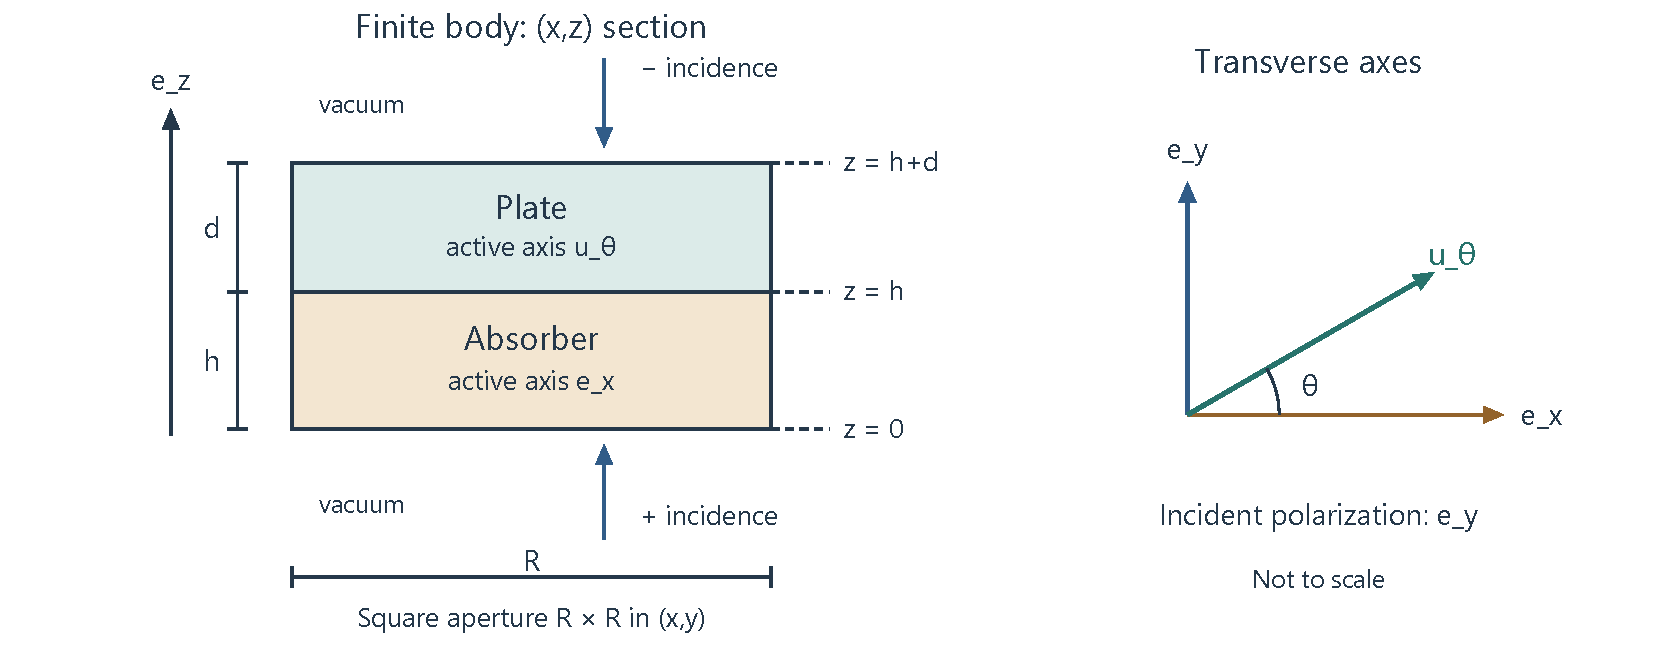
\includegraphics[width=\linewidth]{figures/two-layer-geometry.pdf}
\caption{Finite two-layer geometry and transverse material axes, not to scale. Both incident waves have electric polarization $\ey$. The $+$ wave encounters the absorber first; the $-$ wave encounters the plate first. Each layer has square transverse aperture $R\times R$. The susceptibilities in~\eqref{eq:rankone} are intermediate; adding $i\nu I$ in~\eqref{eq:positive-loss} gives the final strictly lossy tensors.}\label{fig:geometry}
\end{figure}

\subsection{A reflectionless plate under any upper real-permittivity cap}
Given $P>1$, choose an integer $j\geq1$ such that
\begin{equation}\label{eq:plate-design}
 p_j=\left(\frac{2j}{2j-1}\right)^2\leq P,\qquad
 a=p_j-1,\qquad kd=(2j-1)\pi.
\end{equation}
As $j$ increases, $p_j$ decreases to one while $d=(2j-1)\pi/k$ increases: smaller permitted dielectric contrast requires a thicker plate. For each fixed cap $P>1$, choose a permitted integer $j$ once and keep it fixed throughout the construction.

At $\delta=0$, the phase along $\uvec$ is $2j\pi$, and the orthogonal transverse phase is $(2j-1)\pi$. Matching tangential $E,\mathbf H$, equivalently the scalar $E,E'$, gives zero reflection in both principal directions. The boundary-plane Jones transmission and the vacuum plate phase are
\begin{equation}\label{eq:jones}
 H_\theta=2\uvec\uvec^T-I_2,\qquad v_W=e^{ikd}=-1.
\end{equation}
Indeed, propagation of $(E,E'/k)^T$ through a scalar layer of index $n$ is the matrix with entries $\cos(nkd),\sin(nkd)/n,-n\sin(nkd),\cos(nkd)$; at an integer multiple of $\pi$ it is $\pm I_2$.

All slab coefficients are referenced to their boundary planes: unit incident electric amplitude at one interface gives reflected amplitude $r$ there and transmitted amplitude $t$ at the other interface. A vacuum layer of width $\ell$ has $r=0,t=e^{ik\ell}$; write $v_A=e^{ikh}$ for the absorber's vacuum reference phase. For the absorber's $x$ polarization, put $n=\sqrt{1+i\eta}$ on the passive branch, $r_0=(1-n)/(1+n)$, and $p=e^{inkh}$. Its exact amplitudes and absorptance are
\begin{equation}\label{eq:absorber}
 r_A=\frac{r_0(1-p^2)}{1-r_0^2p^2},\qquad
 t_A=\frac{(1-r_0^2)p}{1-r_0^2p^2},\qquad
 A_x=1-\abs{r_A}^2-\abs{t_A}^2.
\end{equation}
$\abs{r_0}<1$ and $\abs p<1$ make the denominator nonzero and $t_A\ne0$. The scalar flux identity $A_x=k\eta\int_0^h\abs{E_x}^2\dd z$ proves $A_x>0$: a zero field inside would force both $1+r_A=0$ and $1-r_A=0$ at the incident interface. Thus $0<A_x<1$.

\begin{lemma}[Regular normalized planar limit]\label{lem:planar}
At zero plate loss and $\sin\theta\ne0$, the physical planar power densities are
\begin{equation}\label{eq:lossless-planar}
 X_\infty=4\sin^2\theta,\qquad
 A_\infty^+=0,\qquad
 A_\infty^-=4\sin^2\theta\cos^2\theta A_x.
\end{equation}
Their normalized values extend to $\theta=0$ with $Y_\infty=4$, $B_\infty^+=0$, $B_\infty^-=4\cos^2\theta A_x$. For fixed finite $h,\eta,j$, the normalized powers are jointly continuous in $(\delta,\theta)$ near $(0,0)$, and
\begin{equation}\label{eq:planar-continuity}
 Y_{\infty,\delta}(0)\to4,\qquad
 \gamma_{\infty,\delta}(0):=
 \frac{\abs{B_{\infty,\delta}^+(0)-B_{\infty,\delta}^-(0)}}{Y_{\infty,\delta}(0)}\to A_x
 \quad(\delta\downarrow0).
\end{equation}
\end{lemma}
\begin{proof}
From the absorber side, $y$ crosses vacuum-equivalent material before the reflectionless plate. From the plate side, $H_\theta\ey$ has $x$ component $\sin2\theta$, giving absorption $\sin^22\theta A_x$. In both directions the co-polar transmission relative to vacuum is $\cos2\theta$. The planar optical theorem is $X_\infty=2(1-\Re t_{\mathrm{co}})$, with scattered transmission defined by subtracting the vacuum wave \citep{Gustafsson2012}. This proves~\eqref{eq:lossless-planar}.

Let $r_W,t_W$ be scalar slab coefficients for permittivity $p_j+i\delta$ and width $d$. Put $D=1-r_Ar_W\cos^2\theta$. Define $t_{\mathrm{co}}$ as the complete-stack co-polar transmitted amplitude divided by the vacuum factor $e^{ik(h+d)}=v_Av_W$. Exact cascade matching gives
\begin{equation}\label{eq:planar-formula}
 t_{\mathrm{co}}=1+\frac{(t_W/v_W-1)\sin^2\theta}{D},\qquad
 Y_{\infty,\delta}(\theta)=2\Re\left\{\frac{1-t_W/v_W}{D}\right\}.
\end{equation}
At $(\delta,\theta)=(0,0)$, $r_W=0,t_W=1,D=1$. Appendix~\ref{app:amplitudes} supplies every scattered amplitude divided by $\sin\theta$ as a nonsingular continuous expression. Squared norms give the continuous normalized scattering, and $B_\infty=Y_\infty-C_\infty$ gives continuous absorption. This proves~\eqref{eq:planar-continuity} without dividing two vanishing quantities.
\end{proof}
Finally take $\eta=1/N$ and $kh=N^2$. Then $r_0\to0$, while $\abs p=\exp[-N^2\Im\sqrt{1+i/N}]\to0$, since $N\Im\sqrt{1+i/N}\to1/2$. Hence $A_x\to1$. Every selected $h,\eta$ is finite and positive; $j$ stays fixed for the cap $P$.

\section{Uniform physical-aperture estimates}\label{sec:aperture}
Write $L=h+d$ and $\mathcal H=L^2((0,L))$. The planar scalar operator uses the same $J_\theta,\alpha,w$, now on the interval. Let $K_{\boldsymbol\kappa}$ be the transverse Fourier fiber of the vector Green operator, and set
\begin{equation}\label{eq:fibers}
 B_{\boldsymbol\kappa,\theta}=J_\theta^*K_{\boldsymbol\kappa}J_\theta,\qquad
 r_{\infty,\theta}^\pm=(\alpha^{-1}-B_{\mathbf0,\theta})^{-1}g_\pm.
\end{equation}
The planar $Y_\infty,B_\infty^\pm,C_\infty^\pm$ are given by the normalized work formulas on $(0,L)$, per unit area. They are dimensionless; $Y_R,B_R,C_R$ have units of area. The auxiliary planar response at angle zero is not the physical zero-angle illumination.

\begin{theorem}[Uniform normalized aperture limit]\label{thm:aperture}
Fix $k,h,d,\eta,a,\delta>0$ and a compact angle interval $I_\theta$. Extend $r_{\infty,\theta}^\pm$ constantly in the transverse coordinates. As $R\to\infty$,
\begin{equation}\label{eq:aperture-current}
 \sup_{\theta\in I_\theta}\frac{\norm{r_{R,\theta}^\pm-r_{\infty,\theta}^\pm}_{L^2(D_R)}}{R}\longrightarrow0.
\end{equation}
Uniformly on $I_\theta$,
\begin{equation}\label{eq:aperture-power}
 \frac{Y_R}{R^2}\to Y_\infty,\qquad
 \frac{B_R^\pm}{R^2}\to B_\infty^\pm,\qquad
 \frac{C_R^\pm}{R^2}\to C_\infty^\pm.
\end{equation}
The auxiliary ratios converge uniformly as well. These statements include arbitrary sequences $\theta_R\to0$ in $I_\theta$. Constants may depend on the fixed thicknesses and positive active losses; no joint uniformity as those losses vanish or thicknesses diverge is asserted.
\end{theorem}

\subsection{Weyl fibers and the grazing singularity}
Use $\widehat v(\boldsymbol\kappa)=\int_{\mathbb R^2}e^{-i\boldsymbol\kappa\cdot\mathbf x}v(\mathbf x)\dd\mathbf x$, with inverse factor $(2\pi)^{-2}$. Let
\begin{equation}\label{eq:weyl}
 \beta(\boldsymbol\kappa)=\sqrt{k^2-\abs{\boldsymbol\kappa}^2},\qquad
 G_{\boldsymbol\kappa}(z)=\frac{i}{2\beta(\boldsymbol\kappa)}e^{i\beta(\boldsymbol\kappa)\abs z},
\end{equation}
on the outgoing/decaying branch. For transverse indices $a,b\in\{1,2\}$,
\begin{equation}\label{eq:weyl-blocks}
 \begin{aligned}
 (K_{\boldsymbol\kappa})_{ab}&=(k^2\delta_{ab}-\kappa_a\kappa_b)G_{\boldsymbol\kappa}*,\\
 (K_{\boldsymbol\kappa})_{a3}&=(K_{\boldsymbol\kappa})_{3a}=i\kappa_a\partial_zG_{\boldsymbol\kappa}*,\\
 (K_{\boldsymbol\kappa})_{33}&=\abs{\boldsymbol\kappa}^2G_{\boldsymbol\kappa}*-I.
 \end{aligned}
\end{equation}
Convolution integrates the source height over $(0,L)$. These formulas follow by transverse Fourier transformation of $( -\Delta-k^2)g_k=\delta_0$. In particular, $\partial_z^2G_{\boldsymbol\kappa}=-\beta^2G_{\boldsymbol\kappa}-\delta_0$ supplies the longitudinal local term.

Since $\abs G\leq(2\abs\beta)^{-1}$ and $\abs{\partial_zG}\leq1/2$ off the diagonal, Schur estimates yield finite constants depending on $k,L$ such that
\begin{equation}\label{eq:fiber-bounds}
 \begin{aligned}
 \norm{K_{\boldsymbol\kappa}}&\leq C\left(1+\abs{\boldsymbol\kappa}
       +\frac{k^2+\abs{\boldsymbol\kappa}^2}{\abs{\beta(\boldsymbol\kappa)}}\right),\\
 \norm{K_{\boldsymbol\kappa}-K_{\mathbf0}}&\leq C_1\abs{\boldsymbol\kappa},
       \qquad\abs{\boldsymbol\kappa}\leq k/2.
 \end{aligned}
\end{equation}
The second bound follows from bounded derivatives of the kernels on the low-frequency disk. The possible grazing singularity is $\big\lvert\abs{\boldsymbol\kappa}-k\big\rvert^{-1/2}$, locally integrable in two dimensions; its square need not be integrable. At zero transverse wavevector the active transverse kernel is $(ik/2)e^{ik\abs{z-z'}}$ times the dot product of the active axes. Its imaginary quadratic form is a positive sum of the two outgoing planar fluxes. Thus the planar inverse has the same bound $c_0^{-1}$ and $\norm{r_{\infty,\theta}^\pm}\leq c_0^{-1}\norm{g_\pm}$ uniformly in angle.

\subsection{Mixed Fourier localization proof}
\begin{proof}[Proof of Theorem~\ref{thm:aperture}]
Choose a fixed $v\in C_c^\infty((-1/2,1/2)^2)$ and put $v_R(\mathbf x)=v(\mathbf x/R)$. Extend $J_\theta$ constantly in the transverse coordinates on $\mathbb R^2\times(0,L)$. For a compactly supported strip current $p$, define the unrestricted observation field $\mathcal Kp=(k^2I+\nabla\nabla\cdot)(g_k*\widetilde p)$, where $\widetilde p$ is its zero extension in three dimensions. For $r\in\mathcal H$, set $\widetilde H_{R,\theta}=J_\theta^*\mathcal K(J_\theta(v_Rr))-v_RB_{\mathbf0,\theta}r$ on this strip and $H_{R,\theta}=\widetilde H_{R,\theta}|_{D_R}$. The latter equals $J_\theta^*K_{D_R}J_\theta(v_Rr)-v_RB_{\mathbf0,\theta}r$ on $D_R$. The global auxiliary field has transverse Fourier representation
\begin{equation}\label{eq:commutator}
 \widehat{\widetilde H}_{R,\theta}(\boldsymbol\kappa)
 =R^2\widehat v(R\boldsymbol\kappa)(B_{\boldsymbol\kappa,\theta}-B_{\mathbf0,\theta})r.
\end{equation}
First derive this identity for smooth compactly supported height profiles by the distributional Weyl formula. The transverse transform acts on the global auxiliary field before aperture restriction. Density extends the distributional identity to $\mathcal H$ and the following estimates to its aperture restriction.

For $\abs{\boldsymbol\kappa}\leq k/2$, Hilbert-valued Plancherel and~\eqref{eq:fiber-bounds} bound the global $L^2$ norm of the low-frequency part of $\widetilde H_{R,\theta}$ by $C\norm r\norm{\nabla v_R}_2=C\norm r\norm{\nabla v}_2$. For the complementary region choose an integer $N>3$. Schwartz decay gives $R^2\abs{\widehat v(R\boldsymbol\kappa)}\leq C_{v,N}R^{2-N}\abs{\boldsymbol\kappa}^{-N}$, and
\begin{equation}\label{eq:grazing-integral}
 \int_{\abs{\boldsymbol\kappa}>k/2}\abs{\boldsymbol\kappa}^{-N}
 (\norm{K_{\boldsymbol\kappa}}+\norm{K_{\mathbf0}})\dd\boldsymbol\kappa<\infty.
\end{equation}
The grazing part is locally $L^1$; at infinity the radial integrand is $O(\rho^{2-N})$. Inverse Fourier $L^1$ control gives the complementary part of $\widetilde H_{R,\theta}$ a transverse $L^\infty(\mathcal H)$ bound $C_{v,N}R^{2-N}\norm r$. Restricting to the aperture gives an $L^2(D_R)$ bound $C_{v,N}R^{3-N}\norm r$. Therefore
\begin{equation}\label{eq:commutator-bound}
 \norm{H_{R,\theta}}_{L^2(D_R)}\leq C_v\norm r+o(1)\norm r
\end{equation}
uniformly in angle, because each $J_\theta$ is an isometry. Only the low-frequency part used global Plancherel. For the density passage, boundedness of the restricted $K_{D_R}$ identifies the local $L^2$ limit with the volume field; the high-frequency inverse transforms converge in transverse $L^\infty(\mathcal H)$. Thus no square of the grazing singularity is introduced.

Take $r=r_{\infty,\theta}^\pm$. The trial current has residual $(v_R-1)g_\pm-H_{R,\theta}$ in~\eqref{eq:scalar}. Apply~\eqref{eq:scalar-inverse} and compare $v_Rr$ with the constant transverse extension of $r$:
\begin{equation}\label{eq:current-error}
 \sup_{\theta\in I_\theta}\frac{\norm{r_{R,\theta}^\pm-r_{\infty,\theta}^\pm}_{L^2(D_R)}}{R}
 \leq C\norm{1-v}_{L^2((-1/2,1/2)^2)}+\frac{C_v}{R}+o(R^{-1}).
\end{equation}
At fixed $v$, let $R\to\infty$; then approximate one in $L^2$ by such smooth windows. The left side is independent of the window, proving~\eqref{eq:aperture-current}. The material aperture and incident field were never smoothed.

Both exact and planar-extended currents have norm $O(R)$ uniformly in angle. Cauchy--Schwarz in the work formula gives $\abs{Y_R-R^2Y_\infty}=o(R^2)$. Boundedness of $w$ and the quadratic-form difference estimate give $\abs{B_R^\pm-R^2B_\infty^\pm}=o(R^2)$. Exact energy balance gives the scattering limit by subtraction. This controls the full integrated scattering, including edge radiation and a narrowing forward peak.

The zero-wavevector operator varies continuously in norm with $\theta$; its uniformly bounded inverse makes the planar powers continuous. Positive $w$ and nonzero $g_\pm$ imply $Y_\infty>0$, so its minimum on $I_\theta$ is positive. Division therefore gives uniform convergence of the auxiliary ratios, including the zero-angle limit.
\end{proof}

\section{Exact prescribed-extinction realization}\label{sec:realization}
\subsection{A root in a finite rank-one object}
Fix $0<\epsilon<1$. Choose a finite absorber with $0<\eta<Q/3$ and $A_x>1-\epsilon/4$. Lemma~\ref{lem:planar} then permits a fixed $0<\delta<Q/3$ such that $\gamma_{\infty,\delta}(0)>1-\epsilon/2$. Choose $\theta_0>0$ so that the planar normalized ratio exceeds $1-5\epsilon/8$ on $[0,\theta_0]$. Freeze these material parameters and thicknesses before enlarging the aperture.

Set $Y_0=Y_{\infty,\delta}(0)>0$ and define
\begin{equation}\label{eq:angle-bracket}
 \theta_{\mathrm{lo}}(R)=\sqrt{\frac{E_*}{2R^2Y_0}},\qquad
 \theta_{\mathrm{hi}}(R)=\sqrt{\frac{2E_*}{R^2Y_0}}.
\end{equation}
For sufficiently large finite $R$ this bracket lies in $(0,\theta_0]$, and the uniform aperture theorem and the exact factorization imply
\begin{equation}\label{eq:endpoints}
 X_R(\theta_{\mathrm{lo}}(R))\to E_*/2,\qquad
 X_R(\theta_{\mathrm{hi}}(R))\to2E_*.
\end{equation}
Indeed, $Y_R(\theta)/R^2\to Y_0$ along either endpoint and $\sin\theta/\theta\to1$. For large $R$, throughout the bracket $\Gamma_R>1-3\epsilon/4$.

At fixed $R$, $J_\theta$ and $L_{R,\theta}$ vary continuously in operator norm; the inverse identity and~\eqref{eq:scalar-inverse} give continuity of $X_R$. The intermediate value theorem supplies an angle $\theta_R\in[\theta_{\mathrm{lo}}(R),\theta_{\mathrm{hi}}(R)]$ with $X_R(\theta_R)=E_*$ exactly. Reciprocity supplies the same extinction for the other incidence. Monotonicity and a nonzero derivative are unnecessary. For every choice of such bracketed roots,
\begin{equation}\label{eq:root-scaling}
 R\theta_R\to\sqrt{E_*/Y_0},\qquad
 \Gamma_R(\theta_R)\to\gamma_{\infty,\delta}(0).
\end{equation}
This scaling is an auxiliary statement about the intermediate rank-one family; it is not a uniform loss-regularized resource estimate.

\subsection{Strict tensor loss without losing the exact target}
For the selected finite $R$, add common isotropic loss:
\begin{equation}\label{eq:positive-loss}
 \chi_{A,\nu}=i\eta\ex\ex^T+i\nu I,\qquad
 \chi_{W,\theta,\nu}=(a+i\delta)\uvec\uvec^T+i\nu I,
 \qquad\nu>0.
\end{equation}
Continuity at the rank-deficient tensor follows from an explicit full-vector electric-field inverse:
\begin{equation}\label{eq:electric-inverse}
 (I-K_{D_R}J_\theta\alpha J_\theta^*)^{-1}
 =I+K_{D_R}J_\theta L_{R,\theta}^{-1}J_\theta^*.
\end{equation}
Multiplication in either order verifies this using $L_{R,\theta}=\alpha^{-1}-J_\theta^*K_{D_R}J_\theta$. The inverse norm is at most $1+\norm{K_{D_R}}/c_0$, uniformly on the compact angle bracket for this fixed body.

Adding $i\nu I$ changes the electric-field operator by $-i\nu K_{D_R}$. If $\nu\norm{K_{D_R}}(1+\norm{K_{D_R}}/c_0)<1$, a Neumann series gives an inverse converging uniformly to~\eqref{eq:electric-inverse} as $\nu\downarrow0$. Fields, currents, and their finite-domain power forms are consequently continuous in $(\nu,\theta)$ uniformly on the bracket. Its unperturbed extinction has a positive minimum, so the normalized ratio is uniformly continuous there too.

Choose $0<\nu<Q/3$ small enough to preserve both strict endpoint inequalities around $E_*$ and $\Gamma>1-\epsilon$ everywhere in the bracket. A second intermediate-value argument gives a possibly adjusted angle with $X_+=X_-=E_*$ exactly. In the absorber, the real eigenvalues are all one and the loss eigenvalues are $\eta+\nu,\nu,\nu$. In the plate the real eigenvalues are $p_j,1,1$ and the loss eigenvalues are $\delta+\nu,\nu,\nu$. They obey~\eqref{eq:material}. The finite object has strictly positive tensor loss and satisfies~\eqref{eq:main}; Lemma~\ref{lem:strict} supplies its strict upper bound. Letting $\epsilon\downarrow0$ proves both suprema in~\eqref{eq:suprema}.

The order of choices matters: choose a finite absorber, choose positive active plate loss, fix an angle interval, enlarge the aperture, and only then choose isotropic loss and retune. None of the estimates is asserted uniform in a vanishing active loss or a diverging thickness. The main theorem needs preservation of the bracket, not a quantitative rate for the final angle.

\section{Physical consequences and limitations}\label{sec:consequences}
At fixed extinction, label the more absorbing incidence $\mathrm{hi}$ and the other one $\mathrm{lo}$. Energy balance gives
\begin{equation}\label{eq:deficit}
 1-\Gamma=\frac{S_{\mathrm{hi}}+A_{\mathrm{lo}}}{E_*}.
\end{equation}
Thus $\Gamma\to1$ implies $A_{\mathrm{hi}}\to E_*$, $S_{\mathrm{hi}}\to0$, $A_{\mathrm{lo}}\to0$, and $S_{\mathrm{lo}}\to E_*$. No finite member has zero $S_{\mathrm{hi}}$ at positive extinction. Define co-polar forward directivity by
\begin{equation}\label{eq:directivity}
 D_{\mathrm{co},\mathrm{hi}}=\frac{4\pi\abs{\ey^\dagger F_{\mathrm{hi}}(\mathbf d_{\mathrm{hi}})}^2}{S_{\mathrm{hi}}},\qquad
 \Gamma\leq1-\frac{k^2E_*}{4\pi D_{\mathrm{co},\mathrm{hi}}},\qquad\mathbf d_{\mathrm{hi}}=\pm\ez.
\end{equation}
The inequality follows by squaring the forward optical theorem and using $\abs{\Im z}\leq\abs z$. It is an established efficiency/directivity obstruction, consistent with the antenna literature \citep{AndersenFrandsen2005}. The expanding aperture permits the required unbounded directivity and a narrowing forward peak.

The selected positive principal-axis susceptibilities are compatible with passive causal scalar dispersion at the chosen frequency. For a target $a+ib$ with $a\geq0,b>0$, choose any $\gamma>0$ and set
\begin{equation}\label{eq:lorentz}
 \chi(\zeta)=\frac{F}{\omega_0^2-\zeta^2-i\gamma\zeta},\qquad
 \omega_0^2-\omega^2=\frac{a}{b}\gamma\omega,\qquad
 F=\gamma\omega\frac{a^2+b^2}{b}>0.
\end{equation}
Then $\chi(\omega)=a+ib$. Independent oscillators on the real principal axes preserve locality and reciprocity. This compatibility observation is not part of the formal main theorem and gives no bandwidth claim.

This one-frequency matching does not automatically preserve~\eqref{eq:material} throughout a band: for example, the $a=0$ oscillator has negative real susceptibility immediately above the matching frequency. For a fixed causal realization with continuous outgoing response and positive extinction at the design frequency, continuity preserves any strict contrast threshold on some neighborhood, with extinction close to its design value. That neighborhood can depend on the device and shrink along an extremizing sequence; it need not contain a band prescribed in advance.

A prescribed-band extension instead fixes $B=[\omega_1,\omega_2]$, with $0<\omega_1<\omega_c<\omega_2$, before choosing the device. One geometry, orientation and complete passive causal reciprocal dielectric law must serve the whole band, with the illumination pair~\eqref{eq:incident} evaluated at $k=\omega/c$ and the material conditions~\eqref{eq:material} imposed at every $\omega\in B$. A useful extinction requirement is
\[
 X(\omega_c)=E_*,\qquad
 \inf_{\omega\in B}X(\omega)\geq E_{\min},\qquad
 0<E_{\min}\leq E_*.
\]
Exact center-frequency tuning and a positive band floor are distinct requirements; neither specifies a constant extinction spectrum.

For a resource-constrained version, fix a bounded enclosing region $D_0$ and an admissible family $\mathcal M$ of complete material dispersion laws. Retaining the two-layer geometry class, suppose the laws satisfy the bandwise conditions above and give well-posed continuous responses. For a nonempty admissible class, define
\[
 G_B(D_0,\mathcal M;E_*,E_{\min})=
 \sup_{\substack{D\subset D_0,\ \varepsilon\in\mathcal M\\
 X(\omega_c)=E_*,\ \inf_{\omega\in B}X(\omega)\geq E_{\min}}}
 \ \inf_{\omega\in B}\Gamma(\omega).
\]
Each term in the outer supremum uses one fixed body and dispersion law. For continuous responses with positive worst-case contrast, $A_+-A_-$ has constant sign on the connected band, so the more absorbing side cannot switch within it.

Two different extensions remain outside this theorem: whether the unit worst-case supremum survives on a prescribed band with only bandwise upper material caps and no common geometric bound or positive loss floor, and the sharp value of $G_B$ for a fixed resource class. A frequencywise resource ceiling $\Gamma(\omega)\leq U(\omega)$ already implies $G_B\leq\inf_{\omega\in B}U(\omega)$; an additional causal tradeoff must go beyond that ceiling and account for one jointly realizable dispersion law. No gap caused by bandwidth alone is asserted here. Extending the present construction would require frequency-uniform aperture and loss-regularization estimates, and control of the extinction floor with one center-frequency retuning. Requiring $X(\omega)=E_*$ throughout $B$ is a separate stronger condition. These broadband formulations are outlook questions, not additional proved or formally verified results.

The theorem supplies no practical finite-size optimizer, quantitative universal resource cost, common positive loss floor, or all-isotropic realization. Aperture and absorber thickness can grow, and the final isotropic loss can shrink. The fixed-resource and quartic small-object questions require different quantifiers and remain separate.

\section{Formal verification correspondence}\label{sec:formal}
The accompanying Lean 4 formalization is frozen at commit
\begin{center}\small\texttt{686402a6c2d63820828729cc7ab02504632e3fe7}.\end{center}
Its principal declaration is
\begin{quote}
\texttt{OQ7Prescribed.theorem11\_complete}\\
\texttt{: PhysicalTheorem11Statement}.
\end{quote}
It proves the prescribed-extinction existence statement, both exact suprema, well-posedness for the admissible two-layer class, physical optical identities, reciprocal extinction and strict nonattainment. The formal material conditions, geometry and cross-section definitions match those of Sections~\ref{sec:model} and~\ref{sec:main}. Weak fields are identified almost everywhere; radiation and sphere-flux limits use the canonical exterior representative.

Supplement S1 records the statement correspondence and distinguishes direct formal declarations, mathematical consequences and exposition not separately formalized. The formal localization proof and the Weyl-fiber presentation in Section~\ref{sec:aperture} use different organizations. The correspondence of the main theorem does not certify every intermediate estimate or paragraph of this manuscript's proof presentation. The causal-dispersion observation in Section~\ref{sec:consequences} also lies outside the formal main theorem.

The archived final AI-assisted audit examines the frozen declaration and reports kernel validity, semantic fidelity to the original main theorem and lemma, Maxwell correctness within the formal model, both suprema and strict nonattainment. The version mapping identifies these statements with Theorem~\ref{thm:main} and Lemma~\ref{lem:strict}. The main declaration depends only on \texttt{propext}, \texttt{Classical.choice} and \texttt{Quot.sound}. The recorded fresh replay uses Lean's own kernel implementation. Kernel checking certifies the encoded statement; the supplied semantic assessment is AI-assisted and does not constitute human peer review or an independently implemented kernel check.

\noindent\textbf{Code and verification materials.}
Frozen proof sources and statement correspondence accompany this article as ancillary files in the \path{anc} directory. They comprise the source archive
\begin{center}\small\path{OQ7-complete-physical-theorem11-source.zip}\end{center}
and \path{THEOREM_CORRESPONDENCE.md}. The ancillary manifest, final audit report, status summary and provenance identify the exact source version and the scope of its verification. Historical checking records retain their original dates and scope; they do not certify every paragraph of this manuscript. No experimental or simulation datasets are used.

\noindent\textbf{AI assistance.}
AI assistance was used for document preparation, source-to-claim comparison, compilation checks and focused literature-priority analysis. The accompanying mathematical and semantic reviews are AI-assisted.

\section{Conclusion}\label{sec:conclusion}
The prescribed-extinction problem has a unit normalized supremum within finite compact two-layer reciprocal anisotropic dielectrics at one frequency and under arbitrary fixed positive upper material caps. The proof combines exact rotation factorization, uniform normalized aperture localization, and two finite-object continuity arguments. Each selected object retains the exact extinction target and strictly positive tensor loss, while strict optical-theorem nonattainment prevents equality for an individual body. This establishes the resource-unrestricted supremum for the stated formulation of OQ7; finite-resource optima and bandwidth remain separate questions.

\appendix
\section{Entire outgoing weak vacuum uniqueness}\label{app:weak}
This appendix supplies the converse-representation step without assuming classical traces of arbitrary weak representatives. Let $E,\mathbf H\in H_{\mathrm{loc}}(\mathrm{curl})$ solve the vacuum equations~\eqref{eq:maxwell} on all of $\mathbb R^3$ and satisfy~\eqref{eq:outgoing}. Choose a smooth radial cutoff $\eta_R$ equal to one on $r\leq R$ and zero on $r\geq2R$, with $w_R=-\eta_R'\geq0$ and $\int_R^{2R}w_R\dd r=1$. Weighted weak Green identities follow by local mollification, compact integration by parts, and passage to the limit in products of local $L^2$ fields. The constant-coefficient curls commute with mollification; the products converge in $L^1$. In particular, the real Poynting identity gives
\begin{equation}\label{eq:weak-energy}
 \int_{\mathbb R^3}w_R\Re\{E\cdot\overline{\mathbf H\times\mathbf n}\}\dd\mathbf x=0,
 \quad\mathbf n=\mathbf x/\abs{\mathbf x}.
\end{equation}
The pointwise norm-square identity and outgoing condition yield
\begin{equation}\label{eq:weak-shell}
 \int w_R\bigl(\norm E^2+\norm{\mathbf H\times\mathbf n}^2\bigr)
 =\int w_R\norm{\mathbf H\times\mathbf n-E}^2=o(1),
\end{equation}
since $\int w_R/r^2\dd\mathbf x=4\pi$.

For an arbitrary $q\in C_c^\infty(\mathbb R^3)^3$, let $(E_q,\mathbf H_q)$ be its outgoing volume fields, so $\nabla\times\mathbf H_q=-ik(E_q+q)$. These smooth fields satisfy $E_q=O(r^{-1})$ and $\mathbf H_q\times\mathbf n-E_q=O(r^{-2})$ outside the source support. The weak bilinear Lorentz identity, derived by the same compact product argument, is
\begin{equation}\label{eq:weak-lorentz}
 ik\int\eta_R E\cdot q\dd\mathbf x
 =\int w_R\{E\cdot(\mathbf H_q\times\mathbf n)
                  -E_q\cdot(\mathbf H\times\mathbf n)\}\dd\mathbf x.
\end{equation}
Rewrite the integrand as $E\cdot(\mathbf H_q\times\mathbf n-E_q)-E_q\cdot(\mathbf H\times\mathbf n-E)$. Cauchy--Schwarz and~\eqref{eq:weak-shell} bound the first term by $o(1)O(R^{-1})$, using $\int w_R/r^4\dd\mathbf x\leq4\pi/R^2$. The second tends to zero by $E_q=O(r^{-1})$, uniform outgoing decay, and $\int w_R/r^2\dd\mathbf x=4\pi$. For large $R$, $\eta_R=1$ on the fixed source support, so $\int E\cdot q=0$ for every smooth compact vector test. Distributional injectivity gives $E=0$ almost everywhere, and its curl equation gives $\mathbf H=0$ almost everywhere.

For a general weak scattering state, subtract the compact-source reconstruction with $p=\chi E$. The difference is an entire outgoing vacuum pair and hence vanishes. This proves the converse representation before applying constitutive volume-equation uniqueness. It also explains why equality of arbitrary raw weak representatives is stated almost everywhere, while the smooth exterior representative carries the pointwise radiation and flux limits.

\section{Nonsingular normalized planar amplitudes}\label{app:amplitudes}
The reference planes are $L:z=0$ and $R:z=L=h+d$. For $b^+$ and $b^-$ the incident $y$ amplitude is one at the left and right planes, respectively. The latter convention multiplies $f_-$ by $e^{ikL}$, an overall unit-modulus phase that does not change powers. Outgoing amplitudes are read at these planes. Let $s=\sin\theta$, $c=\cos\theta$, $v_A=e^{ikh}$, $v_W=e^{ikd}$, $\Delta=t_W-v_W$, and $D=1-r_Ar_Wc^2$. With output order $(Lx,Ly,Rx,Ry)$, subtract $v_Av_W\ey$ from the transmitted amplitude and divide the scattered vector by $s$. Cascade matching gives
\begin{equation}\label{eq:amplitudes-plus}
 b^+=\frac1D\begin{pmatrix}
 r_Wv_At_Ac\\r_Wv_A^2s\\cv_A(\Delta+v_Wr_Ar_W)\\sv_A\Delta
 \end{pmatrix},
\end{equation}
\begin{equation}\label{eq:amplitudes-minus}
 b^-=\begin{pmatrix}
 ct_A\Delta/D\\sv_A\Delta/D\\
 c\{r_A\Delta(v_W+\Delta c^2)/D+r_W\}\\
 s\{r_A\Delta^2c^2/D+r_W\}
 \end{pmatrix}.
\end{equation}
The scalar amplitudes are obtained by matching $E,E'$ at the two boundaries of each layer; the common denominator sums the reflected $x$-channel feedback $r_Ar_Wc^2$. All expressions extend continuously at $s=0$ near $\delta=0$, where $D=1$. The normalized powers are $C_\infty^\pm=\norm{b^\pm}^2$ and $B_\infty^\pm=Y_\infty-C_\infty^\pm$. Substituting $r_W=0,t_W=1,v_W=-1$ gives $C_\infty^+=4$ and $C_\infty^-=4(s^2+c^2(\abs{r_A}^2+\abs{t_A}^2))$, recovering Lemma~\ref{lem:planar} directly.

An operator argument independently justifies this regular limit. At $\delta=0$ the active scalar susceptibility stays nonzero. The projected transverse planar Green kernel on the finite interval is Hilbert--Schmidt, so $\alpha^{-1}-B_{\mathbf0,\theta}$ is Fredholm of index zero. A nullvector reconstructs a source-free outgoing passive one-dimensional field. Its flux identity forces both outgoing amplitudes to vanish; exterior $E,E'$ are therefore zero at an interface. Uniqueness of the finite-layer ordinary differential equation makes the field and current zero. The inverse exists, and operator-norm perturbation gives joint continuity in $(\delta,\theta)$ near $(0,0)$ for the fixed auxiliary drives. No inverse estimate uniform as $\delta\downarrow0$ is used in the aperture theorem.

\small
\bibliographystyle{unsrtnat}
\bibliography{references}
\end{document}
